\documentclass[../main.tex]{subfiles}
\graphicspath{
    {"../img/"}
    {"img/"}
}

\begin{document}
Ostatnio skończyliśmy na kroku $n-1\to n$ i wiemy, że dla $n-1$ wymiarów możemy napisać $\int_{A\in \mathbb{R}^{n-1}}f(x)dx = \int_{B\in \mathbb{R}^{n-1}}f(\xi(t)) |\det \xi'|dt$
\begin{figure}[h]
    \centering
    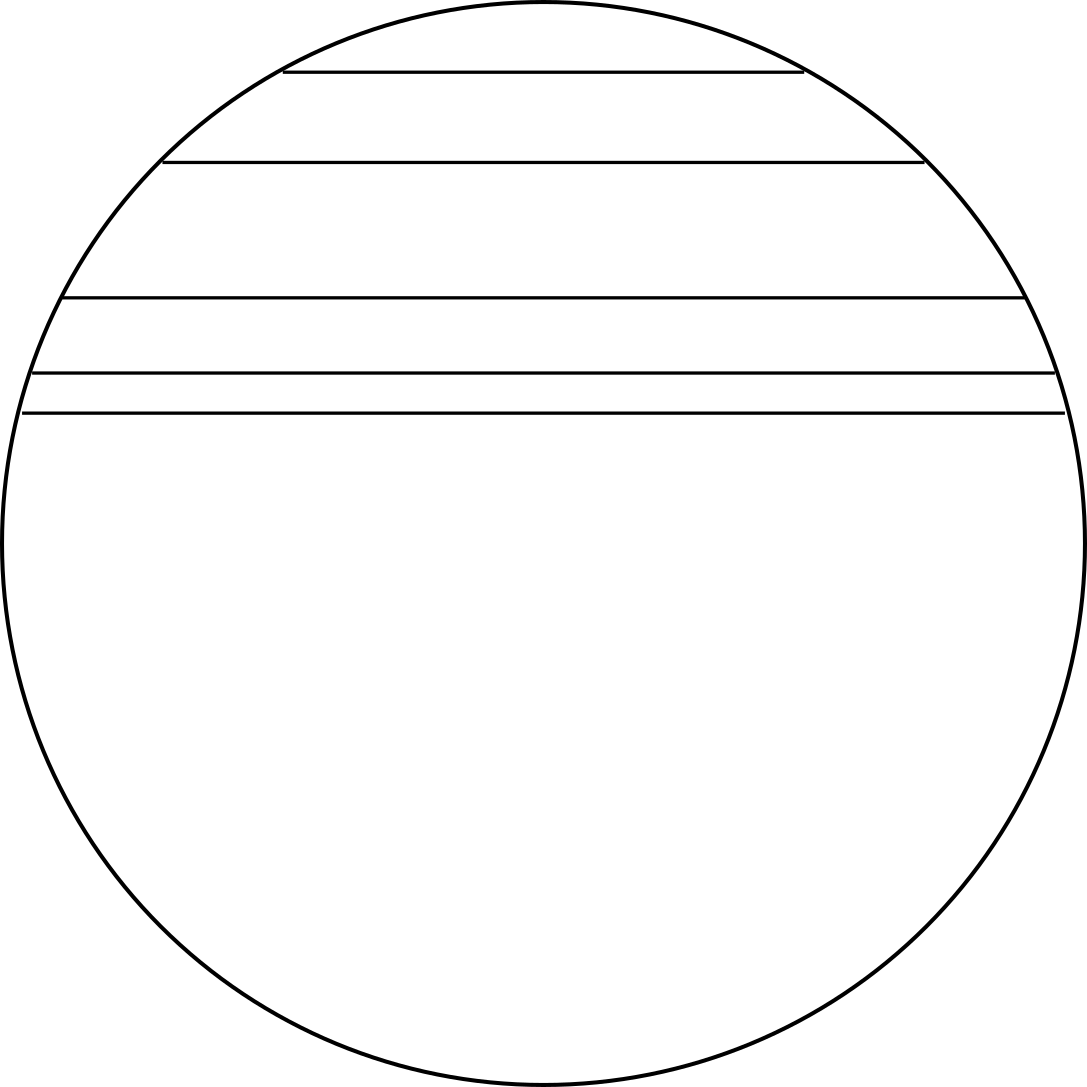
\includegraphics[width=0.3\textwidth]{fig_48}
    \caption{Kółko $K$ składamy z kresek $K_a$ i mamy $\int_K f = \int da \int_{K_a} f$}
    \label{fig:fig_48}
\end{figure}
\[
    \int_{\Theta} f dx = \int_{\Omega}f(\xi(t))|\det \xi'|dt
.\]
Mając zbiór $\Theta$, zdefiniujmy zbiór $\Theta_a$, który jest zbiorem takich $x\in\Theta$, że na miejsca $x_i$ wstawimy wielkość $a$.
\[
    \Theta_a = \left\{ x\in \mathbb{Q}, x = \left( x^1,x^2,\ldots,x^{i-1},a,x^{i+1},\ldots,x^n \right)  \right\}
.\]
\[
    K = \left\{ (x,y), x^2+y^2 = 1 \right\}
.\]
\[
    K_a = \left\{ (x,y)\in K, (x,y) = (x,a) \right\}, \left\{ (x,a), x^2+a^2 = 1 \right\}
.\]
Oznacza to, że
\[
    \int_\Theta f dx = \int da \int_{Theta_a}f(x^1,x^2,\ldots,x^{i-1},a,x^{i+1},\ldots,x^n) dx^1 dx^2 \ldots dx^{i-1} dx^{i+1}\ldots dx^n
.\]
Rozważmy $\xi: \Theta \to \Omega$ taką, że
\[
    \begin{bmatrix} t_1\\ \vdots \\ t_n \end{bmatrix} \to \begin{bmatrix} \xi_1(t_1,\ldots,t_n)\\ \xi_2(t_1,\ldots,t_n) \\ \vdots \\ \xi_{i-1} \\ t_1 \\ \xi_{i+1} \\ \vdots \\ \xi_n(t_1,\ldots,t_n)
\end{bmatrix} \begin{bmatrix} x^1\\x^1\\ \vdots \\ x^i \\ \vdots \\ x^n \end{bmatrix}
.\]
(Czyli $\xi$ nie zmienia jednej współrzędnej np. $\begin{bmatrix} x\\y \end{bmatrix} \to \begin{bmatrix} r\\x \end{bmatrix} $ ).\\
Możemy więc zapisać transformację $\xi_a: \Theta_a\to\Omega_a$
 \[
     \begin{bmatrix} t_1\\ \vdots\\ t_{i-1}\\ t_{i+1} \\ \vdots \\ t_n \end{bmatrix} \to \begin{bmatrix} \xi_1(t_1,\ldots,t_n) \\ \xi_2(t_1,\ldots,t_n) \\ \vdots \\ \xi_{i-1}(\ldots) \\ \xi_{i+1}(\ldots) \\ \vdots \\ \xi_n(t_1,\ldots,t_n)\end{bmatrix}
.\]
Wówczas na mocy założenia indukcyjnego wiemy, że
\begin{align*}
    &\int_{\Theta_a}f(x^1,\ldots,x^{i-1},a,x^{i+1},\ldots,x^n) dx^1 \ldots dx^{i-1} dx^{i+1} \ldots dx^n = \\
    &\int_{\Omega_a} f(t_1,t_2,\ldots,t_{i-1},a,t_{i+1},\ldots,t_n) |\det \xi'_a | dt^1 dt_2 \ldots dt^{i-1} dt^{i+1} \ldots dt^n
.\end{align*}
Wówczas
\begin{align*}
    &\int_{\Theta}f(x^1,\ldots,x^n)dx^n = \int_a da \int_{\Omega_a}f(t_1,\ldots,t_{i-1},a,t_{i+1},\ldots,t_n) |\det \xi'_a| \cdot (\pm 1) dt^1 \ldots dt^{i-1} dt^{i+1} \ldots dt^n\\
    &= \begin{bmatrix} a=t_i \end{bmatrix} =\\
    &= \int_{\Omega} f(t^1,t^2,\ldots,t^n)|\det \xi' | dt^1 \ldots dt^n\quad\Box
.\end{align*}
\[
    \xi' = \begin{bmatrix} \frac{\partial \xi_1}{\partial t_1} & \frac{\partial \xi_2}{\partial t_2} & \ldots && \frac{\partial \xi_n}{\partial t_n}\\ 0 & \ldots & 1 & \ldots & 0 \\ \frac{\partial \xi_n}{\partial t_1} & \ldots &&& \frac{\partial \xi_n}{\partial t_n}  \end{bmatrix}
.\]
\begin{przyklad}
    Policzmy całkę $I = \int_0^{\infty}e^{-x^2}dx$. Nie umiemy. Ale skoro nie umiemy policzyć $I$, to tym bardziej $I^2?$
    \[
        I^2 = \int_0^{\infty}e^{-x^2}dx \int_0^{\infty}e^{-y^2}dy = \int_{\Box} e^{-(x^2+y^2)}
    .\]
    Zamieńmy sobie zmienne: $x = r\cos \varphi,\quad y = r\sin \varphi$. $\psi: \begin{bmatrix} r\\\varphi\end{bmatrix}\to \begin{bmatrix} x\\y \end{bmatrix}  $, $|\psi'| = r$
     Mamy
     \begin{align*}
         &I^2 = \int_0^{\infty}dr \int_0^{\frac{\pi}{2}}d\varphi e^{-r^2}r = \frac{\pi}{2} \lim\limits_{p\to +\infty} \int_0^p dr \cdot e^{-r^2} \cdot r = \frac{\pi}{2} \lim\limits_{p\to\infty} \left[ -\frac{1}{2}e^{-r^2} \right] _0^p\\
         &\frac{\pi}{2}\left[ \lim\limits_{p\to\infty}\left[ -\frac{1}{2}e^{-p^2} \right] - \left[ -\frac{1}{2}e^{(0)^2} \right]  \right] = \frac{\pi}{2} \frac{1}{2} = \frac{\pi}{4}
     \end{align*}
     czyli $I^2 = \frac{\pi}{4} \implies I = \frac{\sqrt{\pi} }{2}$
\end{przyklad}
\subsection{Formy różniczkowe}
(czyli o uprawianiu analizy na powierzchni balonika albo kartki)

Niech $M\subset\mathbb{R}^n$ - taki, że dla każdego punktu $p\in M$ istnieje otoczenie otwarte $U\subset M$
\begin{przyklad}
    (sfera, obwarzanek, itd., okrąg), (stożek - nie ok!), (taka ósemka co się przecina - też nie)
    TODO: obrazki
\end{przyklad}
\begin{definicja}
Niech $U$ - zbiór otwarty $\subset M$ i niech odwzorowanie $\varphi: U\to \mathbb{R}^n$ takie, że $\varphi$ - klasy $\mathcal{C}^1$, (czasami $\mathcal{C}^\infty$ ), $\varphi^{-1}$ - klasy $\mathcal{C}^1$, (czasami $\mathcal{C}^\infty$ ) nazywamy mapą.\\
Uwaga: mapa \underline{nie musi} pokrywać całego zbioru $M$.
\end{definicja}

Wyobraźmy sobie, że mamy jakiś zbiór $M$. Połowa tego zbioru to niech będzie $U_1$, i ono się przecina z $U_2$. $U_1$ i $U_2$ możemy rozłożyć na prostokąty w $\mathbb{R}^2$. Co się stanie z punktami mapowanymi do obu $U$?
\begin{definicja}
    $(U^1,\varphi^1), (U^2,\varphi^2)$ - mapy na $M$.\\
    $U_1$ i $U_2$ nazywamy zgodnymi jeżeli\\
    $a)$ $U_1\cap U_2 = \phi$\\
    albo odwzorowanie $\varphi_2 \circ \varphi_1^{-1}: \varphi_1(U_1\cap U_2)\to \varphi_2(U_2\cap U_1)$ jest bijekcją (klasy powiedzmy sobie $\mathcal{C}^1, \mathcal{C}^{\infty}$ )
\end{definicja}
    \begin{figure}[h]
        \centering
        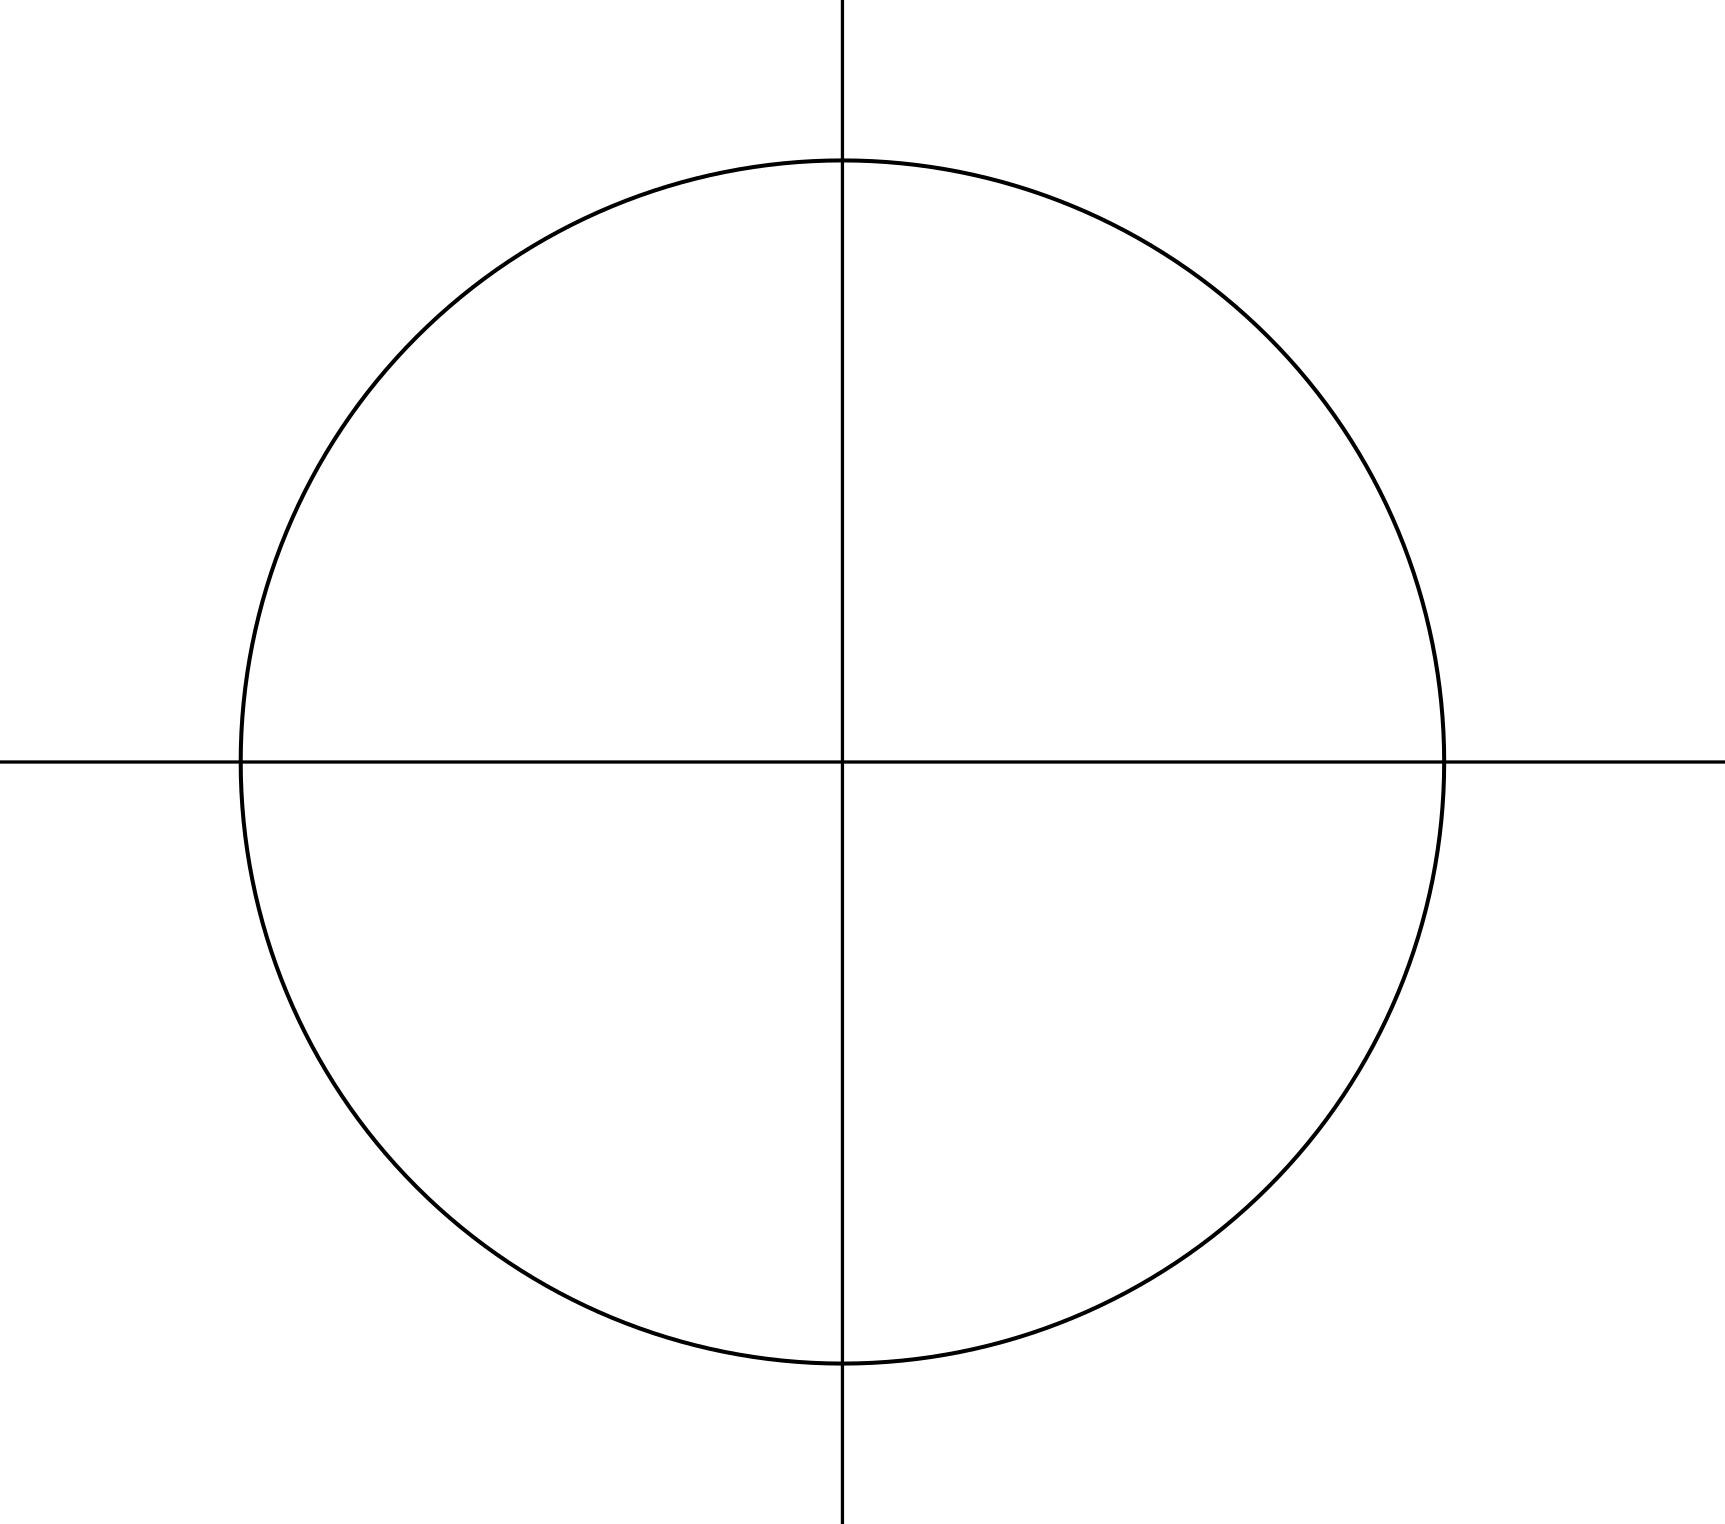
\includegraphics[width=0.5\textwidth]{fig_49}
        \caption{$M = \left\{ (x,y): x^2 + y^2 = 1^2 \right\}$}
    \end{figure}
\begin{przyklad}
    \begin{align*}
    &U_1 = \left\{ (x,y)\in M, y>0 \right\},\quad \varphi_1: (x,y)\in U_1 \to x\\
    &U_2 = \left\{ (x,y)\in M, x>0 \right\},\quad \varphi_2: (x,y)\in U_2 \to y\\
    &U_3 = \left\{ (x,y)\in M, y<0 \right\},\quad \varphi_3: (x,y)\in U_3 \to x\\
    &U_4 = \left\{ (x,y)\in M, x<0 \right\},\quad \varphi_4: (x,y)\in U_4 \to y
    .\end{align*}
    $U_1$ i $U_3$ oraz $U_2$ i $U_4$ są zgodne. Czy zgodne są $U_1$ i $U_2$? Czyli chcemy zbadać odwzorowanie $\varphi_1(U_1\cap U_2)\to \varphi_2(U_1\cap U_2)$, ale $\varphi_1(x,y)\in U_1\to x$.\\
    Czyli $\varphi_1^{-1}(x)\to \left( x, \sqrt{1-x^2}  \right) $,\\
    czyli $\varphi_2(\varphi_1^{-1}(x) = \varphi_2((x,\sqrt{1-x^2} )) = \sqrt{1-x^2} $.\\
    Zatem czy $\varphi_2 \circ \varphi_{-1}^{-1}(x) = \sqrt{1-x^2} $ przerzuca $]0,1[\to]0,1[$ jest różniczkowalne? Odpowiedź: na zbiorze $]0,1[$ jest.
\end{przyklad}
\begin{definicja}
    Kolekcję zgodnych map nazywamy atlasem. Zbiór $M$ wraz z atlasem, który pokrywa cały $M$ nazywamy \textbf{rozmaitością} (\textit{ang. manifold}).
\end{definicja}

\end{document}

